\documentclass[a4paper,norsk]{article}
\usepackage[utf8]{inputenc}
\usepackage[T1]{fontenc,url}
\usepackage{babel,textcomp}
\usepackage{graphicx}
\usepackage{amsmath}
\usepackage{cleveref}
\usepackage[cmyk]{xcolor}
\usepackage{listings}

\lstset {language=C++,    
backgroundcolor=\color{yellow!20},    
commentstyle=\color{green},    
%keywordstyle=\color{blue},    
basicstyle=\footnotesize}
\urlstyle{sf}
\title{Oblig 1 ADS101}
\date{\today}
\author{Adam Aske}
\newpage
\begin{document}
\maketitle
\tableofcontents
\newpage

\section{Introduksjon}
Her bruker jeg algoritmen Selection Sort og C++ sin innnebygde funskjon Sort til å sortere arrayer av forskjellige størrelser. 
Chrono tar tiden på hvor lang tid det tar for arrayer av forskjellige størrelser. 
Målingene er gjennomsnittet av algorytmene som har blitt kjørt 10 ganger per N.

\section{Inorder Traversal}
Inorder traversal vil printe venstre node, root og høyre node. Dette skjer ved at vi går helt ned i venstre gren, når det da ikke er flere venstre noder å besøke,
besøker den rooten og besøker høyre node. Dette gjentar til det ikke er flere noder i treet.
Først skjekker vi om ``current'' har en GetLeft(), hvis den ikke har det printer vi denne noden vi er på og fortsetter til høyre node. 
Dersom vi finner en venstre node lagrer vi denne i ``previous''. Vi går da gjennom alle høyre noder den har og setter det som ny ``previous'' peker.
 Hvis ``previous'' ikke  har noe høyre node, setter vi dens høyre til current for å lagre pekeren som vi kan returnere til senere, så gjentar stegene. 
 Dersom den har en høyre ndoe, printer vi denne og setter den nye current til denne høyre noden og gjentar stegene. 
\begin{lstlisting}[language=C++, caption={Oblig2.cpp}]
void Inorder(BinaryNode* root) {
    BinaryNode* current, *previous;
    current = root;

    while(current != nullptr) {
        //Goes down the left, until there is no more to the left, then goes down right until there is no more
        if (current->GetLeft() != nullptr) {
            previous = current->GetLeft();
            //Get the bottom right and stores it in previous
            while (previous->GetRight() != nullptr && previous->GetRight() != current) {
                previous = previous->GetRight();
            }
            //Here it has gotten the bottom right it can, without a left
            //Store this in previous 
            if (previous->GetRight() == nullptr) {
                //Store the current as previous->Right
                previous->right = current;
                //Then go down the left as long as it goes
                current = current->GetLeft();
            }
            else {
                //If the previous has no right, then print it
                std::cout << current->GetData() << " ";
                //Get the new current as this ones right
                current = current->GetRight();
                //Then returns to check if it has a left, then it prints it
            }
        }
        else {
            //Get the right instead of the left
            std::cout << current->GetData() << " ";
            current = current->GetRight();
        }
    }
}
\end{lstlisting}


\section{Postorde Traversal}
Postorder besøker rooten først, så besøker den vesntre og høyre node. 
Jeg bruker en stack til å utføre denne traversalen.
Først pusher jeg root til stacken, den vil da være Top() i stacken. Så lenge stacken ikke er tom, vil disse stegene gjenta seg.
I loppen lagrer jeg en peker til Top() fra stacken. Så printer vi verdien noden har, vi er da ferdige med denne og popper den ut av stacken.
Så pusher jeg venstre og høyre node hvis rooten har det. Så gjentar jeg stegene til stacken er tom, alle vil da være besøkt. 
\begin{lstlisting}[language=C++, caption={Oblig2.cpp}]
void Postorder(BinaryNode* root)
{
    Stack<BinaryNode*> stack;
    stack.Push(root);

    while (!stack.Empty()) {
        BinaryNode* current = stack.Top();
        stack.Pop();

        std::cout << current->GetData() << " ";

        if (current->GetLeft()) {
            stack.Push(current->GetLeft());
        }

        if (current->GetRight()) {
            stack.Push(current->GetRight());
        }
    }
}
\end{lstlisting}

\section{Amount of Nodes}
For å finne antall noder i treet, gjør jeg nesten det samme som en Postorder traversal. 
Jeg lager en int som heter count, som da blir plusset på 1 hver gang den har besøkt en node. 
Stegene jeg gjør er nøyaktig de samme som Postorder utenom at jeg sier ``count'++'' istedet for å printe verdien til noden.
\begin{lstlisting}[language=C++, caption={Oblig2.cpp}]
int AmountOfNodes(BinaryNode* root)
{
	Stack<BinaryNode*> stack;
	stack.Push(root);

    int count = 0;

    while (!stack.Empty()) 
    {
		BinaryNode* current = stack.Top();
		stack.Pop();
        
        	count++;

		if (current->GetLeft()) {
			stack.Push(current->GetLeft());
		}

		if (current->GetRight()) {
			stack.Push(current->GetRight());
		}
    }
    return count;
}
\end{lstlisting}
\section{Amount of Levels}
Denne funksjonen fungerer veldig likt som Postorder og Amount of Nodes.
For å bare telle nivåer istedenfor noder så laget jeg en bool som heter hasCounted. Denne holder telling på om det er blitt talt dette nivået. 
Hvergang den pusher en ny node til stacken sjekker den om den har allerede telt dette nivået, hvis ikke så tell og pluss på count. 
Den da returnerer count som antall nivåer i treet.
\begin{lstlisting}[language=C++, caption={Oblig2.cpp}]
int AmountOfLevels(BinaryNode* root)
{
	Stack<BinaryNode*> stack;
	stack.Push(root);

	int count = 0;
	bool hasCounted = false;
	while (!stack.Empty()) {
		BinaryNode* current = stack.Top();
		stack.Pop();
       	hasCounted = false;
		
        	//Only add count if it hasnt done it already
		if (current->GetLeft()) {
			stack.Push(current->GetLeft());
            		count++;
            		hasCounted = true;
		}

		if (current->GetRight()) {
			stack.Push(current->GetRight());
            		if (!hasCounted) {
                	count++;
                	hasCounted = true;
            		}
		}
	}
    return count;
}
\end{lstlisting}
\section{Balance Check}
Denne funksjonen fungerer veldig likt som Postorder og Amount of Nodes.
For å bare telle nivåer istedenfor noder så laget jeg en bool som heter hasCounted. Denne holder telling på om det er blitt talt dette nivået. 
Hvergang den pusher en ny node til stacken sjekker den om den har allerede telt dette nivået, hvis ikke så tell og pluss på count. 
Den da returnerer count som antall nivåer i treet.
\begin{lstlisting}[language=C++, caption={Oblig2.cpp}]
bool BalancedCheck(BinaryNode* root)
{
    //Return true if this is null
    if (!root) {
        return true;
    }
    //Find how many levels there is down from here for both left and right
    int leftHeight = Height(root->GetLeft());
    int rightHeight = Height(root->GetRight());
    //The heights must be either 0, then check this for every level of the tree
    //if any level is not balanced the whole loop returns false
    if ((leftHeight - rightHeight) <= 0 && BalancedCheck(root->GetLeft()) && BalancedCheck(root->GetRight())) {
        return true;
    }
    else {
		return false;
    }
    
}
\end{lstlisting}
\begin{lstlisting}[language=C++, caption={Oblig2.cpp}]
int Height(BinaryNode* root) {
    if (!root) {
        return 0;
    }
    else {
        //Goes down the 
        int a = Height(root->GetLeft());
        int b = Height(root->GetRight());

        //returns the highest of the two
        if (a > b) {
            return 1 + a;
        }
        else {
            return 1 + b;
        }
    }
}
\end{lstlisting}
\section{Resultater av binary tree funksjonene.} 
Bilde av binary treet som blir brukt:\newline
\begin{figure}
	\centering
	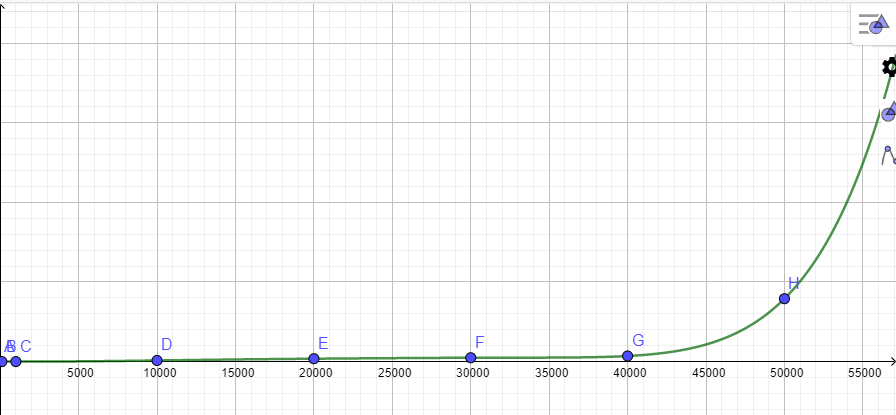
\includegraphics[width =3in]{StdSortGraph.png}
	\caption{X-Aksen er antall elementer i arrayet og Y-Aksen er tiden det tokk for å sortere elementene etter størrelse}
\end{figure}
Inorder Traversal resultat: 1, 2, 4, 7, 8, 10, 16\newline
Postorder Traversal resultat: 7, 10, 16, 8, 2, 4, 1\newline
Amount of Nodes: 7\newline
Amount of Levels: 3\newline
Balanced Check: 1 (0 = Unlbalanced, 1 = Balanced)\newline
\end{document}